\documentclass{vgtc}                          % final 

%% to provide the the path and extension of a graphics file:
%% \includegraphics{diamondrule} is completely sufficient.
%%
\ifpdf%                                % if we use pdflatex
  \pdfoutput=1\relax                   % create PDFs from pdfLaTeX
  \pdfcompresslevel=9                  % PDF Compression
  \pdfoptionpdfminorversion=7          % create PDF 1.7
  \ExecuteOptions{pdftex}
  \usepackage{graphicx}                % allow us to embed graphics files
  \DeclareGraphicsExtensions{.pdf,.png,.jpg,.jpeg} % for pdflatex we expect .pdf, .png, or .jpg files
\else%                                 % else we use pure latex
  \ExecuteOptions{dvips}
  \usepackage{graphicx}                % allow us to embed graphics files
  \DeclareGraphicsExtensions{.eps}     % for pure latex we expect eps files
\fi%

%% it is recomended to use ``\autoref{sec:bla}'' instead of ``Fig.~\ref{sec:bla}''
\graphicspath{{figures/}{pictures/}{images/}{./}} % where to search for the images

\usepackage{microtype}                 % use micro-typography (slightly more compact, better to read)
\PassOptionsToPackage{warn}{textcomp}  % to address font issues with \textrightarrow
\usepackage{textcomp}                  % use better special symbols
\usepackage{mathptmx}                  % use matching math font
\usepackage{times}                     % we use Times as the main font
\renewcommand*\ttdefault{txtt}         % a nicer typewriter font
\usepackage{cite}                      % needed to automatically sort the references
\usepackage{tabu}                      % only used for the table example
\usepackage{booktabs}                  % only used for the table example
\usepackage{url}

%% OnlineID. Otherwise, you may safely leave it at ``0''.
\onlineid{0}

%% declare the category of your paper, only shown in review mode
\vgtccategory{Research}

%% allow for this line if you want the electronic option to work properly
\vgtcinsertpkg

%% In preprint mode you may define your own headline.
%\preprinttext{To appear in an IEEE VGTC sponsored conference.}

%% Paper title.

\title{M4: Final Submission}

%% This is how authors are specified in the conference style

%% Author and Affiliation (single author).
%%\author{Roy G. Biv\thanks{e-mail: roy.g.biv@aol.com}}
%%\affiliation{\scriptsize Allied Widgets Research}

%% Author and Affiliation (multiple authors with single affiliations).
%%\author{Roy G. Biv\thanks{e-mail: roy.g.biv@aol.com} %
%%\and Ed Grimley\thanks{e-mail:ed.grimley@aol.com} %
%%\and Martha Stewart\thanks{e-mail:martha.stewart@marthastewart.com}}
%%\affiliation{\scriptsize Martha Stewart Enterprises \\ Microsoft Research}

%% Author and Affiliation (multiple authors with multiple affiliations)
\author{Nicole Cherches\\
\scriptsize Matr. Nr.: 01506832
\and Alexander Gelb\\
\scriptsize Matr. Nr.: 01268620
\and Benjamin Neckam\\
\scriptsize Matr. Nr.: 01301917
\and Axynia Tokareva\\
\scriptsize Matr. Nr.: 01268620
}

%% A teaser figure can be included as follows, but is not recommended since
%% the space is now taken up by a full width abstract.
%\teaser{
%  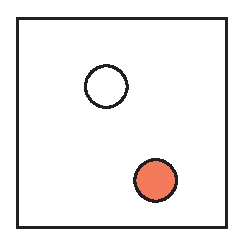
\includegraphics[width=1.5in]{sample.eps}
%  \caption{Lookit! Lookit!}
%}

%% Abstract section.
\abstract{
Some blabla here
} % end of abstract

%% ACM Computing Classification System (CCS). 
%% See <http://www.acm.org/about/class> for details.
%% We recommend the 2012 system <http://www.acm.org/about/class/class/2012>
%% For the 2012 system use the ``\CCScatTwelve'' which command takes four arguments.
%% The 1998 system <http://www.acm.org/about/class/class/2012> is still possible
%% For the 1998 system use the ``\CCScat'' which command takes four arguments.
%% In both cases the last two arguments (1998) or last three (2012) can be empty.

\CCScatlist{
  \CCScatTwelve{Visu\-al\-iza\-tion}{Visu\-al\-iza\-tion techniques}{}{};
  \CCScatTwelve{GAIA}{ESA}{}{}
}

%%%%%%%%%%%%%%%%%%%%%%%%%%%%%%%%%%%%%%%%%%%%%%%%%%%%%%%%%%%%%%%%
%%%%%%%%%%%%%%%%%%%%%% START OF THE PAPER %%%%%%%%%%%%%%%%%%%%%%
%%%%%%%%%%%%%%%%%%%%%%%%%%%%%%%%%%%%%%%%%%%%%%%%%%%%%%%%%%%%%%%%%

\begin{document}

%% The ``\maketitle'' command must be the first command after the
%% ``\begin{document}'' command. It prepares and prints the title block.

%% the only exception to this rule is the \firstsection command
\firstsection{Motivation}
\maketitle
On 19th December 2013 the "European Space Agency", ESA, launched  the "Gaia"-satellite to gather more information about our galaxy and create a three dimensional map out of it. Since then data like velocities, positions, errors, parallax and many more were collected of about 2 million stars. All together each star has 50 features in the data set which means the amount of entries is extremely high.\\
But working with such a huge dataset is not easy and most of the time not necessary because scientists only want to focus on a specific area of the galaxy. Therefore they only use subsets of the data. Now the idea was what happens if we take the whole data set and don't look into detail but see the "big picture" and try to find patterns, correlations, outliers or other interesting things.\\
This could be useful for scientists who are not sure which part of the data they want to explore and for example can focus only on the anomalies or other fascinating sections in the data set.

\section{Related Work}
What we first did, was searching for similar problems and finding out, what other visualizations looked like in this area. Most of the space visualizations we found online, were in 3d. Examples of them are the ESA Star Mapper\footnote{\url{http://sci.esa.int/star\_mapper/}} or 100000 stars\footnote{\url{http://stars.chromeexperiments.com/}}. They both are 3d interactive simulations of the stellar neighbourhood.
We also found a 2d-visualization from the ESA, which visualizes the stars from the Gaia dataset\footnote{\url{https://gea.esac.esa.int/visualization/index.html}}.
But we couldn't find anything that has to do with correlations or patterns. All the existing visualizations were about showing the stars themselves with their exact location.
So we started prototyping and in the end we even used some of our first basic ideas in the end product of out system.
Then we tried to find existing visualization systems. In the VIS course we already learned about Tableau\footnote{\url{https://www.tableau.com/de-de}}, which allows the user to import Data and create visualization plots based on it. And we also found out about a software named Glue\footnote{\url{http://www.glueviz.org/en/stable/}}, which helps to create plots and analyze relationships between different data.
So we basically tried to create a mixture of both tools and started designing our own system.

\begin{figure}[h]
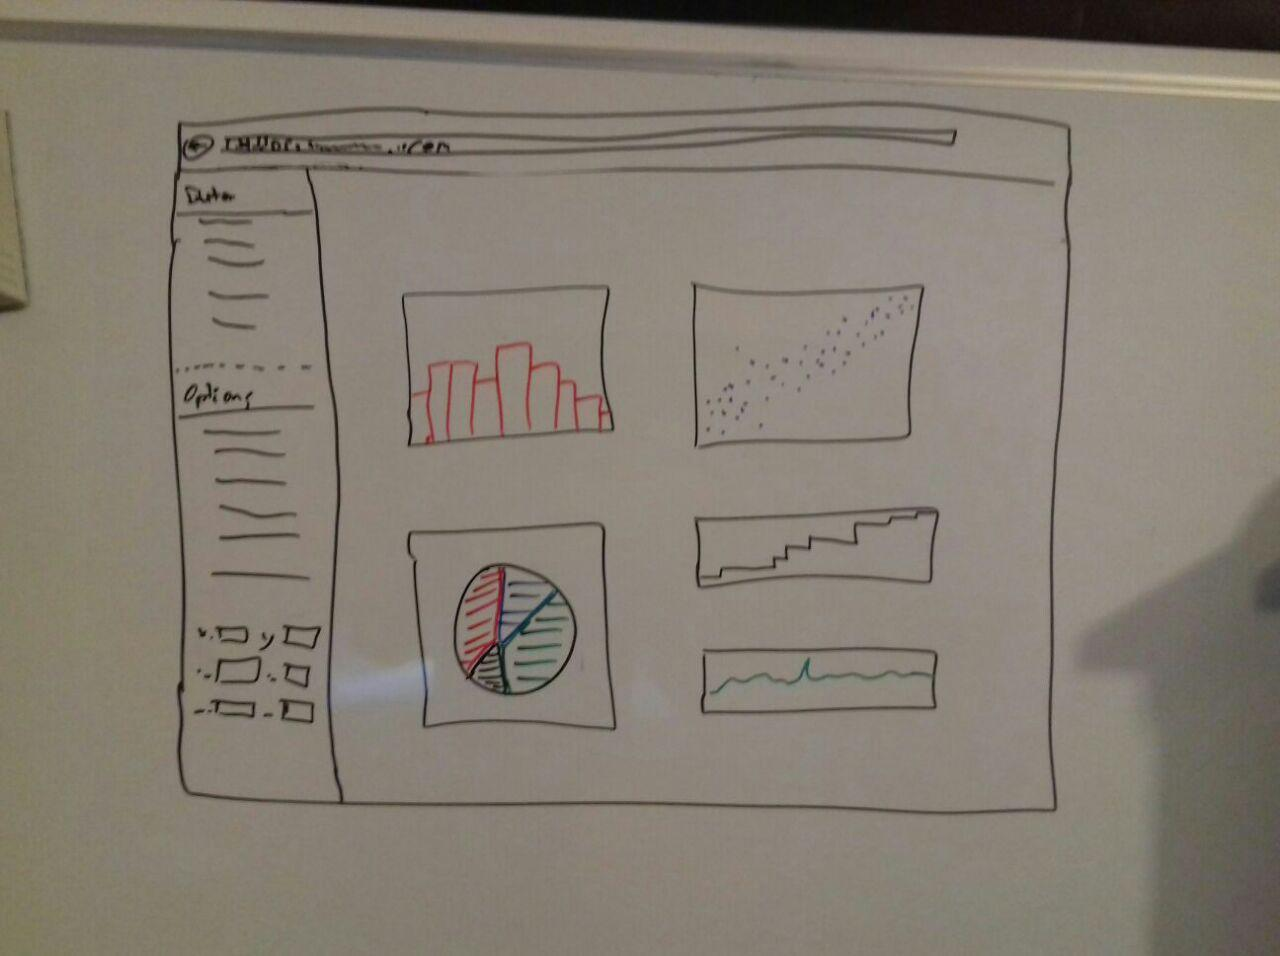
\includegraphics[width=0.5\textwidth]{Prototype1.jpg}
\centering
\caption{Lo-Fi Prototype of our user interface}
\end{figure}

Above is a picture, that shows how we imagined the visualization system at the beginning.
As we will see later in the end product, our Lo-Fi Prototype looks similar to our visualization system. We kept the sidebar, where the user has basic information about the data and can choose options on how the data will be presented. Also the diagrams and plots appear all on one screen so the user can see how they correlate.

\section{Approach}
When we first thought about our visualization design, we tried to think about our user. The system should help to see "the big picture" of a dataset and not only details. So, we thought about plots that could help us to realize that.

What we decided to do, was a Scatterplot Matrix: It really fits into our project, because we can see a whole grid filled with Scatterplots. This way, we can see all Correlations between selected columns of the Dataset.
The user has to choose a set of columns, he wants to analyse in the sidebar. The scatterplot has also histograms in the diagonal, so we can see the patterns even better.

Our system can also be used to compute histograms separately. Here the function creates bins for a specific column and shows how many entrys are in every bin. While hovering over the bars from our plot, we can also see the exact number of those entries.
The user can also set the bin size manually.

Then the system also provides a function to compute a Correlogram. For this, the user has also to select a set of columns. For these columns the function computes and displays the correlation coefficient. So it is easy to see how the different columns of a set are connected and if the user needs to analyse it further.

The last part of the system is the PCA. Blabla über das PCA.

\section{Implementation}
The whole program was written in JavaScript combined with CSS. Therefore it works on every web browser For the front-end we decided to use the toolkit "Bootstrap"\footnote{https://getbootstrap.com/} which provides different templates so we needn't to spend to much time for the user-interface.\\
To visualize the data the JavaScript library "D3"\footnote{https://d3js.org/} was used which offers the ability to let the user interact with the data itself.\\
\\
We encounters many problems which challenged us to implement things properly. One of the problems where to filter the data that all plots can be realized. We figured out that we just can't delete all the entries which contains a NULL or any other non valid values because this would reduce the data set to almost zero entries. Therefore we went through the documentation of the dataset and tried to figure out which features of the stars can be excluded and which not. Unfortunately we can not filter out all unnecessary values at the beginning , we have to do a "pre-filtering" to remove all non integer values and afterwards almost every function has to do their own filtering to adapt the data to their specific task.\\

\section{Results}
We started with making a side bar, which shows a few details about the dataset and allows the user to make some specific settings.
On top, we can see the Dataset name, rows and columns of our dataset.
Firstly, the user can choose which kind of plot he wants to produce in the Options window. 
"Data Value" is a drop down, in which the user can choose exactly one column, which is what we need for the histogram.
If he chooses the Scatterplot, he needs to choose more columns in "Multiple Data".
After that, he clicks the "Plot" Button and the chosen diagram will be visible on the display. With the "Remove" Button, he can clear the page.
\section{Discussion}
\subsection{Lessons learned}
\subsubsection{Benjamin Neckam}
There were two things I will take out of this project.\\
First refers to the implementation and the chosen programming language. Basically I was not very used to JavaScript, to be more precisely I had no experience with it, but I was really impressed by "D3". The opportunities you have to visualize data is breathtaking and allows the programmer to choose over a wide variety of plot types. The only disadvantage that really falls into weight was the performance. If the dataset is bigger than, let's say, 100.000 entries it takes some time to calculate and plot the data and in our case the file contains more than ten times more entries. But all in all it was a very interesting and in my opinion very important for my future to work with JavaScript and "D3" and get deeper into this part of front end programming.\\
The second part is about the collaboration between the project group of the class and research group of another university. Until now all the projects at the university were from the teachers of the faculty itself but in this case the task was from the "Universitätssternwarte Wien". This means we had to arrange meetings with the project leader and a student which also is a member of the research group and talk about the task in detail and what the aim of this project is. It was fun and interesting to meet all these people but I recognized that even if there are not too many people involved it can easily happen that confusion arises. Like in our case, we started to focus on the wrong details and parts and had to "restart" our project. Therefore I would say communication is the most important part in a project, especially if it is a collaboration of two or more groups, I guess this is the biggest lesson I learned from the project. 
\section{Separation of Tasks}
\section{References}


\begin{itemize}
\item If you receive compilation errors along the lines of ``\texttt{Package ifpdf Error: Name clash, \textbackslash ifpdf is already defined}'' then please add a new line ``\texttt{\textbackslash let\textbackslash ifpdf\textbackslash relax}'' right after the ``\texttt{\textbackslash documentclass[journal]\{vgtc\}}'' call. Note that your error is due to packages you use that define ``\texttt{\textbackslash ifpdf}'' which is obsolete (the result is that \texttt{\textbackslash ifpdf} is defined twice); these packages should be changed to use ifpdf package instead.
\item The style uses the hyperref package, thus turns references into internal links. We thus recommend to make use of the ``\texttt{\textbackslash autoref\{reference\}}'' call (instead of ``\texttt{Figure\~{}\textbackslash ref\{reference\}}'' or similar) since ``\texttt{\textbackslash autoref\{reference\}}'' turns the entire reference into an internal link, not just the number. Examples: \autoref{fig:sample} and \autoref{tab:vis_papers}.
\item The style automatically looks for image files with the correct extension (eps for regular \LaTeX; pdf, png, and jpg for pdf\LaTeX), in a set of given subfolders (figures/, pictures/, images/). It is thus sufficient to use ``\texttt{\textbackslash includegraphics\{CypressView\}}'' (instead of ``\texttt{\textbackslash includegraphics\{pictures/CypressView.jpg\}}'').
\item For adding hyperlinks and DOIs to the list of references, you can use ``\texttt{\textbackslash bibliographystyle\{abbrv-doi-hyperref-narrow\}}'' (instead of ``\texttt{\textbackslash bibliographystyle\{abbrv\}}''). It uses the doi and url fields in a bib\TeX\ entry and turns the entire reference into a link, giving priority to the doi. The doi can be entered with or without the ``\texttt{http://dx.doi.org/}'' url part. See the examples in the bib\TeX\ file and the bibliography at the end of this template.\\[1em]
\textbf{Note 1:} occasionally (for some \LaTeX\ distributions) this hyper-linked bib\TeX\ style may lead to \textbf{compilation errors} (``\texttt{pdfendlink ended up in different nesting level ...}'') if a reference entry is broken across two pages (due to a bug in hyperref). In this case make sure you have the latest version of the hyperref package (i.\,e., update your \LaTeX\ installation/packages) or, alternatively, revert back to ``\texttt{\textbackslash bibliographystyle\{abbrv-doi-narrow\}}'' (at the expense of removing hyperlinks from the bibliography) and try ``\texttt{\textbackslash bibliographystyle\{abbrv-doi-hyperref-narrow\}}'' again after some more editing.\\[1em]
\textbf{Note 2:} the ``\texttt{-narrow}'' versions of the bibliography style use the font ``PTSansNarrow-TLF'' for typesetting the DOIs in a compact way. This font needs to be available on your \LaTeX\ system. It is part of the \href{https://www.ctan.org/pkg/paratype}{``paratype'' package}, and many distributions (such as MikTeX) have it automatically installed. If you do not have this package yet and want to use a ``\texttt{-narrow}'' bibliography style then use your \LaTeX\ system's package installer to add it. If this is not possible you can also revert to the respective bibliography styles without the ``\texttt{-narrow}'' in the file name.\\[1em]
DVI-based processes to compile the template apparently cannot handle the different font so, by default, the template file uses the \texttt{abbrv-doi} bibliography style but the compiled PDF shows you the effect of the \texttt{abbrv-doi-hyperref-narrow} style.
\end{itemize}

\section{Bibliography Instructions}

\begin{itemize}
\item Sort all bibliographic entries alphabetically but the last name of the first author. This \LaTeX/bib\TeX\ template takes care of this sorting automatically.
\item Merge multiple references into one; e.\,g., use \cite{Max:1995:OMF,Kitware:2003} (not \cite{Kitware:2003}\cite{Max:1995:OMF}). Within each set of multiple references, the references should be sorted in ascending order. This \LaTeX/bib\TeX\ template takes care of both the merging and the sorting automatically.
\item Verify all data obtained from digital libraries, even ACM's DL and IEEE Xplore  etc.\ are sometimes wrong or incomplete.
\item Do not trust bibliographic data from other services such as Mendeley.com, Google Scholar, or similar; these are even more likely to be incorrect or incomplete.
\item Articles in journal---items to include:
  \begin{itemize}
  \item author names
	\item title
	\item journal name
	\item year
	\item volume
	\item number
	\item month of publication as variable name (i.\,e., \{jan\} for January, etc.; month ranges using \{jan \#\{/\}\# feb\} or \{jan \#\{-{}-\}\# feb\})
  \end{itemize}
\item use journal names in proper style: correct: ``IEEE Transactions on Visualization and Computer Graphics'', incorrect: ``Visualization and Computer Graphics, IEEE Transactions on''
\item Papers in proceedings---items to include:
  \begin{itemize}
  \item author names
	\item title
	\item abbreviated proceedings name: e.\,g., ``Proc.\textbackslash{} CONF\_ACRONYNM'' without the year; example: ``Proc.\textbackslash{} CHI'', ``Proc.\textbackslash{} 3DUI'', ``Proc.\textbackslash{} Eurographics'', ``Proc.\textbackslash{} EuroVis''
	\item year
	\item publisher
	\item town with country of publisher (the town can be abbreviated for well-known towns such as New York or Berlin)
  \end{itemize}
\item article/paper title convention: refrain from using curly brackets, except for acronyms/proper names/words following dashes/question marks etc.; example:
\begin{itemize}
	\item paper ``Marching Cubes: A High Resolution 3D Surface Construction Algorithm''
	\item should be entered as ``\{M\}arching \{C\}ubes: A High Resolution \{3D\} Surface Construction Algorithm'' or  ``\{M\}arching \{C\}ubes: A high resolution \{3D\} surface construction algorithm''
	\item will be typeset as ``Marching Cubes: A high resolution 3D surface construction algorithm''
\end{itemize}
\item for all entries
\begin{itemize}
	\item DOI can be entered in the DOI field as plain DOI number or as DOI url; alternative: a url in the URL field
	\item provide full page ranges AA-{}-BB
\end{itemize}
\item when citing references, do not use the reference as a sentence object; e.\,g., wrong: ``In \cite{Lorensen:1987:MCA} the authors describe \dots'', correct: ``Lorensen and Cline \cite{Lorensen:1987:MCA} describe \dots''
\end{itemize}

\section{Example Section}

Lorem\marginpar{\small You can use the margins for comments while editing the submission, but please remove the marginpar comments for submission.} ipsum dolor sit amet, consetetur sadipscing elitr, sed diam
nonumy eirmod tempor invidunt ut labore et dolore magna aliquyam erat,
sed diam voluptua. At vero eos et accusam et justo duo dolores et ea
rebum. Stet clita kasd gubergren, no sea takimata sanctus est Lorem
ipsum dolor sit amet. Lorem ipsum dolor sit amet, consetetur
sadipscing elitr, sed diam nonumy eirmod tempor invidunt ut labore et
dolore magna aliquyam erat, sed diam
voluptua~\cite{Kitware:2003,Max:1995:OMF}. At vero eos et accusam et
justo duo dolores et ea rebum. Stet clita kasd gubergren, no sea
takimata sanctus est Lorem ipsum dolor sit amet. Lorem ipsum dolor sit
amet, consetetur sadipscing elitr, sed diam nonumy eirmod tempor
invidunt ut labore et dolore magna aliquyam erat, sed diam
voluptua. At vero eos et accusam et justo duo dolores et ea
rebum. Stet clita kasd gubergren, no sea takimata sanctus est.

\section{Exposition}

Duis autem vel eum iriure dolor in hendrerit in vulputate velit esse
molestie consequat, vel illum dolore eu feugiat nulla facilisis at
vero eros et accumsan et iusto odio dignissim qui blandit praesent
luptatum zzril delenit augue duis dolore te feugait nulla
facilisi. Lorem ipsum dolor sit amet, consectetuer adipiscing elit,
sed diam nonummy nibh euismod tincidunt ut laoreet dolore magna
aliquam erat volutpat~\cite{Kindlmann:1999:SAG}.

\begin{equation}
\sum_{j=1}^{z} j = \frac{z(z+1)}{2}
\end{equation}

Lorem ipsum dolor sit amet, consetetur sadipscing elitr, sed diam
nonumy eirmod tempor invidunt ut labore et dolore magna aliquyam erat,
sed diam voluptua. At vero eos et accusam et justo duo dolores et ea
rebum. Stet clita kasd gubergren, no sea takimata sanctus est Lorem
ipsum dolor sit amet. Lorem ipsum dolor sit amet, consetetur
sadipscing elitr, sed diam nonumy eirmod tempor invidunt ut labore et
dolore magna aliquyam erat, sed diam voluptua. At vero eos et accusam
et justo duo dolores et ea rebum. Stet clita kasd gubergren, no sea
takimata sanctus est Lorem ipsum dolor sit amet.

\subsection{Lorem ipsum}

Lorem ipsum dolor sit amet (see \autoref{tab:vis_papers}), consetetur sadipscing elitr, sed diam
nonumy eirmod tempor invidunt ut labore et dolore magna aliquyam erat,
sed diam voluptua. At vero eos et accusam et justo duo dolores et ea
rebum. Stet clita kasd gubergren, no sea takimata sanctus est Lorem
ipsum dolor sit amet. Lorem ipsum dolor sit amet, consetetur
sadipscing elitr, sed diam nonumy eirmod tempor invidunt ut labore et
dolore magna aliquyam erat, sed diam voluptua. At vero eos et accusam
et justo duo dolores et ea rebum. Stet clita kasd gubergren, no sea
takimata sanctus est Lorem ipsum dolor sit amet. Lorem ipsum dolor sit
amet, consetetur sadipscing elitr, sed diam nonumy eirmod tempor
invidunt ut labore et dolore magna aliquyam erat, sed diam
voluptua. At vero eos et accusam et justo duo dolores et ea
rebum. 

\begin{table}[tb]
  \caption{VIS/VisWeek accepted/presented papers: 1990--2016.}
  \label{tab:vis_papers}
  \scriptsize%
	\centering%
  \begin{tabu}{%
	r%
	*{7}{c}%
	*{2}{r}%
	}
  \toprule
   year & \rotatebox{90}{Vis/SciVis} &   \rotatebox{90}{SciVis conf} &   \rotatebox{90}{InfoVis} &   \rotatebox{90}{VAST} &   \rotatebox{90}{VAST conf} &   \rotatebox{90}{TVCG @ VIS} &   \rotatebox{90}{CG\&A @ VIS} &   \rotatebox{90}{VIS/VisWeek} \rotatebox{90}{incl. TVCG/CG\&A}   &   \rotatebox{90}{VIS/VisWeek} \rotatebox{90}{w/o TVCG/CG\&A}   \\
  \midrule
	2016 & 30 &   & 37 & 33 & 15 & 23 & 10 & 148 & 115 \\
  2015 & 33 & 9 & 38 & 33 & 14 & 17 & 15 & 159 & 127 \\
  2014 & 34 &   & 45 & 33 & 21 & 20 &   & 153 & 133 \\
  2013 & 31 &   & 38 & 32 &   & 20 &   & 121 & 101 \\
  2012 & 42 &   & 44 & 30 &   & 23 &   & 139 & 116 \\
  2011 & 49 &   & 44 & 26 &   & 20 &   & 139 & 119 \\
  2010 & 48 &   & 35 & 26 &   &   &   & 109 & 109 \\
  2009 & 54 &   & 37 & 26 &   &   &   & 117 & 117 \\
  2008 & 50 &   & 28 & 21 &   &   &   & 99 & 99 \\
  2007 & 56 &   & 27 & 24 &   &   &   & 107 & 107 \\
  2006 & 63 &   & 24 & 26 &   &   &   & 113 & 113 \\
  2005 & 88 &   & 31 &   &   &   &   & 119 & 119 \\
  2004 & 70 &   & 27 &   &   &   &   & 97 & 97 \\
  2003 & 74 &   & 29 &   &   &   &   & 103 & 103 \\
  2002 & 78 &   & 23 &   &   &   &   & 101 & 101 \\
  2001 & 74 &   & 22 &   &   &   &   & 96 & 96 \\
  2000 & 73 &   & 20 &   &   &   &   & 93 & 93 \\
  1999 & 69 &   & 19 &   &   &   &   & 88 & 88 \\
  1998 & 72 &   & 18 &   &   &   &   & 90 & 90 \\
  1997 & 72 &   & 16 &   &   &   &   & 88 & 88 \\
  1996 & 65 &   & 12 &   &   &   &   & 77 & 77 \\
  1995 & 56 &   & 18 &   &   &   &   & 74 & 74 \\
  1994 & 53 &   &   &   &   &   &   & 53 & 53 \\
  1993 & 55 &   &   &   &   &   &   & 55 & 55 \\
  1992 & 53 &   &   &   &   &   &   & 53 & 53 \\
  1991 & 50 &   &   &   &   &   &   & 50 & 50 \\
  1990 & 53 &   &   &   &   &   &   & 53 & 53 \\
  \midrule
  \textbf{sum} & \textbf{1545} & \textbf{9} & \textbf{632} & \textbf{310} & \textbf{50} & \textbf{123} & \textbf{25} & \textbf{2694} & \textbf{2546} \\
  \bottomrule
  \end{tabu}%
\end{table}

\subsection{Mezcal Head}

Lorem ipsum dolor sit amet (see \autoref{fig:sample}), consetetur sadipscing elitr, sed diam
nonumy eirmod tempor invidunt ut labore et dolore magna aliquyam erat,
sed diam voluptua. At vero eos et accusam et justo duo dolores et ea
rebum. Stet clita kasd gubergren, no sea takimata sanctus est Lorem
ipsum dolor sit amet. Lorem ipsum dolor sit amet, consetetur
sadipscing elitr, sed diam nonumy eirmod tempor invidunt ut labore et
dolore magna aliquyam erat, sed diam voluptua. At vero eos et accusam
et justo duo dolores et ea rebum. Stet clita kasd gubergren, no sea
takimata sanctus est Lorem ipsum dolor sit amet. 

\subsubsection{Duis Autem}

Lorem ipsum dolor sit amet, consetetur sadipscing elitr, sed diam
nonumy eirmod tempor invidunt ut labore et dolore magna aliquyam erat,
sed diam voluptua. At vero eos et accusam et justo duo dolores et ea
rebum. Stet clita kasd gubergren, no sea takimata sanctus est Lorem
ipsum dolor sit amet. Lorem ipsum dolor sit amet, consetetur
sadipscing elitr, sed diam nonumy eirmod tempor invidunt ut labore et
dolore magna aliquyam erat, sed diam voluptua. At vero eos et accusam
et justo duo dolores et ea rebum. Stet clita kasd gubergren, no sea
takimata sanctus est Lorem ipsum dolor sit amet. Lorem ipsum dolor sit
amet, consetetur sadipscing elitr, sed diam nonumy eirmod tempor
invidunt ut labore et dolore magna aliquyam erat, sed diam
voluptua. At vero eos et accusam et justo duo dolores et ea
rebum. Stet clita kasd gubergren, no sea takimata sanctus est. Lorem
ipsum dolor sit amet.

\begin{figure}[tb]
 \centering % avoid the use of \begin{center}...\end{center} and use \centering instead (more compact)
 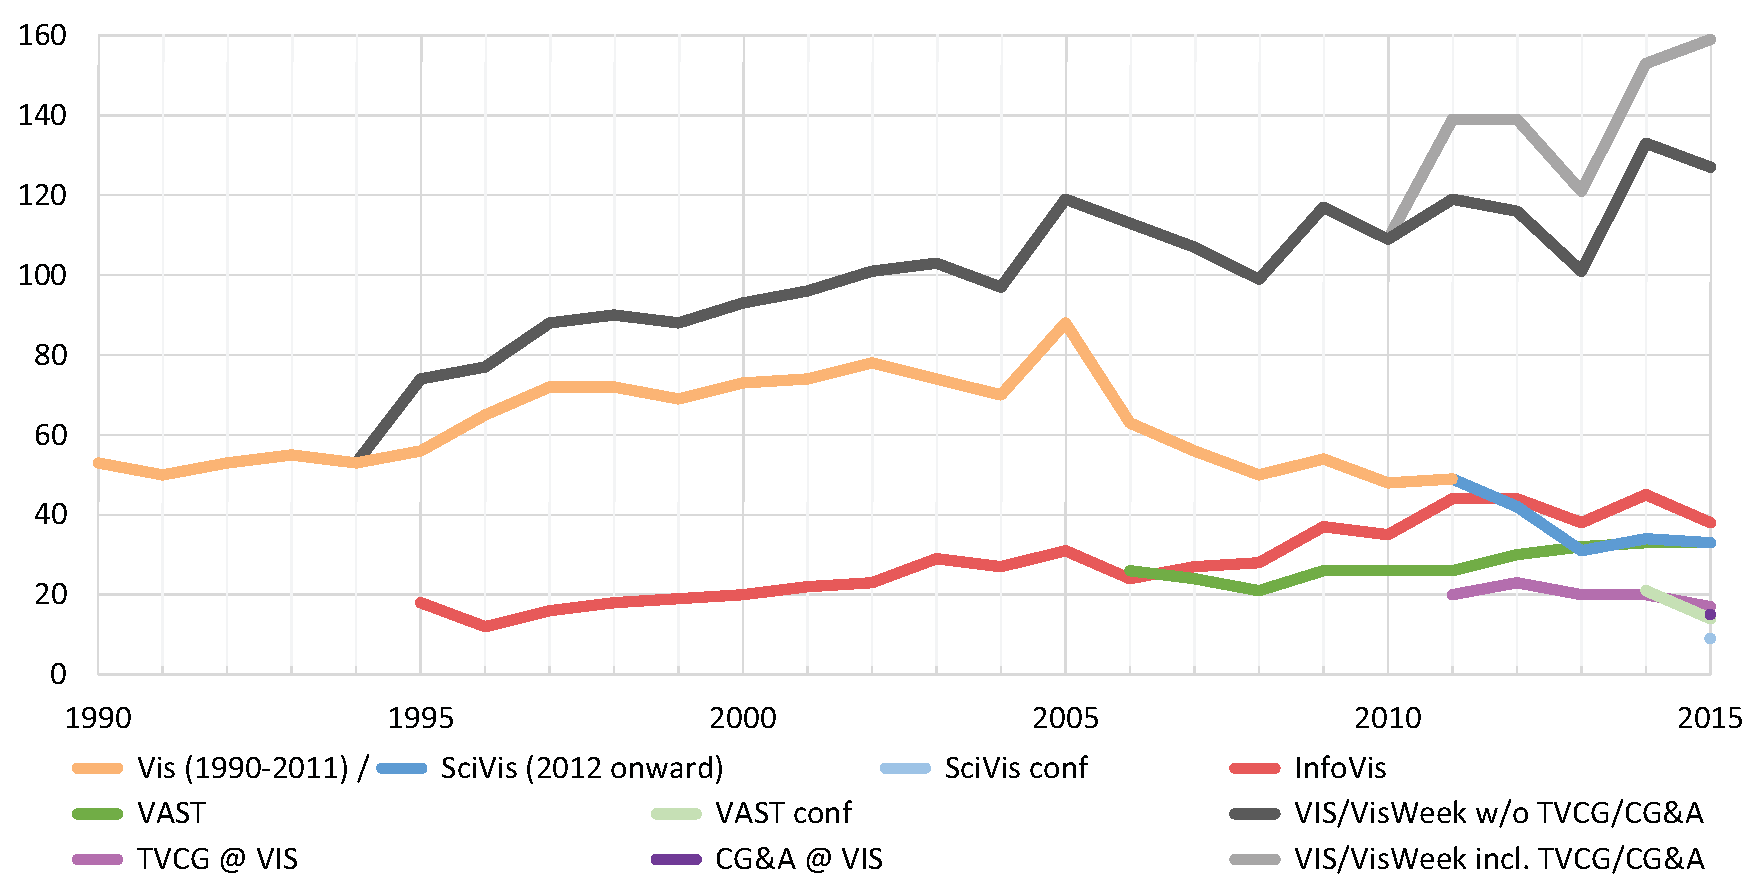
\includegraphics[width=\columnwidth]{paper-count-w-2015-new}
 \caption{A visualization of the 1990--2015 data from \autoref{tab:vis_papers}. The image is from \cite{Isenberg:2017:VMC} and is in the public domain.}
 \label{fig:sample}
\end{figure}

\subsubsection{Ejector Seat Reservation}

Duis autem~\cite{Lorensen:1987:MCA}\footnote{The algorithm behind
Marching Cubes \cite{Lorensen:1987:MCA} had already been
described by Wyvill et al. \cite{Wyvill:1986:DSS} a year
earlier.} vel eum iriure dolor in hendrerit
in vulputate velit esse molestie consequat,\footnote{Footnotes
appear at the bottom of the column.} vel illum dolore eu
feugiat nulla facilisis at vero eros et accumsan et iusto odio
dignissim qui blandit praesent luptatum zzril delenit augue duis
dolore te feugait nulla facilisi. Lorem ipsum dolor sit amet,
consectetuer adipiscing elit, sed diam nonummy nibh euismod tincidunt
ut laoreet dolore magna aliquam erat volutpat.


\paragraph{Confirmed Ejector Seat Reservation}

Ut wisi enim ad minim veniam, quis nostrud exerci tation ullamcorper
suscipit lobortis nisl ut aliquip ex ea commodo
consequat~\cite{Nielson:1991:TAD}. Duis autem vel eum iriure dolor in
hendrerit in vulputate velit esse molestie consequat, vel illum dolore
eu feugiat nulla facilisis at vero eros et accumsan et iusto odio
dignissim qui blandit praesent luptatum zzril delenit augue duis
dolore te feugait nulla facilisi.

\paragraph{Rejected Ejector Seat Reservation}

Ut wisi enim ad minim veniam, quis nostrud exerci tation ullamcorper
suscipit lobortis nisl ut aliquip ex ea commodo consequat. Duis autem
vel eum iriure dolor in hendrerit in vulputate velit esse molestie


\section{Conclusion}

Lorem ipsum dolor sit amet, consetetur sadipscing elitr, sed diam
nonumy eirmod tempor invidunt ut labore et dolore magna aliquyam erat,
sed diam voluptua. At vero eos et accusam et justo duo dolores et ea
rebum. Stet clita kasd gubergren, no sea takimata sanctus est Lorem
ipsum dolor sit amet. Lorem ipsum dolor sit amet, consetetur
sadipscing elitr, sed diam nonumy eirmod tempor invidunt ut labore et
dolore magna aliquyam erat, sed diam voluptua. At vero eos et accusam
et justo duo dolores et ea rebum. Stet clita kasd gubergren, no sea
takimata sanctus est Lorem ipsum dolor sit amet. Lorem ipsum dolor sit
amet, consetetur sadipscing elitr, sed diam nonumy eirmod tempor
invidunt ut labore et dolore magna aliquyam erat, sed diam
voluptua. At vero eos et accusam et justo duo dolores et ea
rebum.


%% if specified like this the section will be committed in review mode
\acknowledgments{
The authors wish to thank A, B, and C. This work was supported in part by
a grant from XYZ.}

%\bibliographystyle{abbrv}
\bibliographystyle{abbrv-doi}
%\bibliographystyle{abbrv-doi-narrow}
%\bibliographystyle{abbrv-doi-hyperref}
%\bibliographystyle{abbrv-doi-hyperref-narrow}

\bibliography{template}
\end{document}